\documentclass[]{article}
\usepackage{lmodern}
\usepackage{amssymb,amsmath}
\usepackage{ifxetex,ifluatex}
\usepackage{fixltx2e} % provides \textsubscript
\usepackage{kotex}
% use upquote if available, for straight quotes in verbatim environments
\IfFileExists{upquote.sty}{\usepackage{upquote}}{}
% use microtype if available
\IfFileExists{microtype.sty}{%
\usepackage{microtype}
\UseMicrotypeSet[protrusion]{basicmath} % disable protrusion for tt fonts
}{}
\usepackage[margin=1in]{geometry}
\usepackage{hyperref}
\hypersetup{unicode=true,
            pdftitle={Chapter2. statistical analysis},
            pdfauthor={Yerim Lim 임예림},
            pdfborder={0 0 0},
            breaklinks=true}
\urlstyle{same}  % don't use monospace font for urls
\usepackage{color}
\usepackage{fancyvrb}
\newcommand{\VerbBar}{|}
\newcommand{\VERB}{\Verb[commandchars=\\\{\}]}
\DefineVerbatimEnvironment{Highlighting}{Verbatim}{commandchars=\\\{\}}
% Add ',fontsize=\small' for more characters per line
\usepackage{framed}
\definecolor{shadecolor}{RGB}{248,248,248}
\newenvironment{Shaded}{\begin{snugshade}}{\end{snugshade}}
\newcommand{\KeywordTok}[1]{\textcolor[rgb]{0.13,0.29,0.53}{\textbf{#1}}}
\newcommand{\DataTypeTok}[1]{\textcolor[rgb]{0.13,0.29,0.53}{#1}}
\newcommand{\DecValTok}[1]{\textcolor[rgb]{0.00,0.00,0.81}{#1}}
\newcommand{\BaseNTok}[1]{\textcolor[rgb]{0.00,0.00,0.81}{#1}}
\newcommand{\FloatTok}[1]{\textcolor[rgb]{0.00,0.00,0.81}{#1}}
\newcommand{\ConstantTok}[1]{\textcolor[rgb]{0.00,0.00,0.00}{#1}}
\newcommand{\CharTok}[1]{\textcolor[rgb]{0.31,0.60,0.02}{#1}}
\newcommand{\SpecialCharTok}[1]{\textcolor[rgb]{0.00,0.00,0.00}{#1}}
\newcommand{\StringTok}[1]{\textcolor[rgb]{0.31,0.60,0.02}{#1}}
\newcommand{\VerbatimStringTok}[1]{\textcolor[rgb]{0.31,0.60,0.02}{#1}}
\newcommand{\SpecialStringTok}[1]{\textcolor[rgb]{0.31,0.60,0.02}{#1}}
\newcommand{\ImportTok}[1]{#1}
\newcommand{\CommentTok}[1]{\textcolor[rgb]{0.56,0.35,0.01}{\textit{#1}}}
\newcommand{\DocumentationTok}[1]{\textcolor[rgb]{0.56,0.35,0.01}{\textbf{\textit{#1}}}}
\newcommand{\AnnotationTok}[1]{\textcolor[rgb]{0.56,0.35,0.01}{\textbf{\textit{#1}}}}
\newcommand{\CommentVarTok}[1]{\textcolor[rgb]{0.56,0.35,0.01}{\textbf{\textit{#1}}}}
\newcommand{\OtherTok}[1]{\textcolor[rgb]{0.56,0.35,0.01}{#1}}
\newcommand{\FunctionTok}[1]{\textcolor[rgb]{0.00,0.00,0.00}{#1}}
\newcommand{\VariableTok}[1]{\textcolor[rgb]{0.00,0.00,0.00}{#1}}
\newcommand{\ControlFlowTok}[1]{\textcolor[rgb]{0.13,0.29,0.53}{\textbf{#1}}}
\newcommand{\OperatorTok}[1]{\textcolor[rgb]{0.81,0.36,0.00}{\textbf{#1}}}
\newcommand{\BuiltInTok}[1]{#1}
\newcommand{\ExtensionTok}[1]{#1}
\newcommand{\PreprocessorTok}[1]{\textcolor[rgb]{0.56,0.35,0.01}{\textit{#1}}}
\newcommand{\AttributeTok}[1]{\textcolor[rgb]{0.77,0.63,0.00}{#1}}
\newcommand{\RegionMarkerTok}[1]{#1}
\newcommand{\InformationTok}[1]{\textcolor[rgb]{0.56,0.35,0.01}{\textbf{\textit{#1}}}}
\newcommand{\WarningTok}[1]{\textcolor[rgb]{0.56,0.35,0.01}{\textbf{\textit{#1}}}}
\newcommand{\AlertTok}[1]{\textcolor[rgb]{0.94,0.16,0.16}{#1}}
\newcommand{\ErrorTok}[1]{\textcolor[rgb]{0.64,0.00,0.00}{\textbf{#1}}}
\newcommand{\NormalTok}[1]{#1}
\usepackage{graphicx,grffile}
\makeatletter
\def\maxwidth{\ifdim\Gin@nat@width>\linewidth\linewidth\else\Gin@nat@width\fi}
\def\maxheight{\ifdim\Gin@nat@height>\textheight\textheight\else\Gin@nat@height\fi}
\makeatother
% Scale images if necessary, so that they will not overflow the page
% margins by default, and it is still possible to overwrite the defaults
% using explicit options in \includegraphics[width, height, ...]{}
\setkeys{Gin}{width=\maxwidth,height=\maxheight,keepaspectratio}
\IfFileExists{parskip.sty}{%
\usepackage{parskip}
}{% else
\setlength{\parindent}{0pt}
\setlength{\parskip}{6pt plus 2pt minus 1pt}
}
\setlength{\emergencystretch}{3em}  % prevent overfull lines
\providecommand{\tightlist}{%
  \setlength{\itemsep}{0pt}\setlength{\parskip}{0pt}}
\setcounter{secnumdepth}{0}
% Redefines (sub)paragraphs to behave more like sections
\ifx\paragraph\undefined\else
\let\oldparagraph\paragraph
\renewcommand{\paragraph}[1]{\oldparagraph{#1}\mbox{}}
\fi
\ifx\subparagraph\undefined\else
\let\oldsubparagraph\subparagraph
\renewcommand{\subparagraph}[1]{\oldsubparagraph{#1}\mbox{}}
\fi

%%% Use protect on footnotes to avoid problems with footnotes in titles
\let\rmarkdownfootnote\footnote%
\def\footnote{\protect\rmarkdownfootnote}

%%% Change title format to be more compact
\usepackage{titling}

% Create subtitle command for use in maketitle
\newcommand{\subtitle}[1]{
  \posttitle{
    \begin{center}\large#1\end{center}
    }
}

\setlength{\droptitle}{-2em}
  \title{Chapter2. statistical analysis}
  \pretitle{\vspace{\droptitle}\centering\huge}
  \posttitle{\par}
  \author{Yerim Lim 임예림}
  \preauthor{\centering\large\emph}
  \postauthor{\par}
  \predate{\centering\large\emph}
  \postdate{\par}
  \date{2018년 2월 1일}


\begin{document}
\maketitle

{
\setcounter{tocdepth}{2}
\tableofcontents
}
\section{기초통계분석}

\subsection{기술통계량}

\paragraph{기술통계량을 구해보자.}\label{-.}

데이터를 살펴보자. 두 개의 변수로 이루어져있고, 각각 몸무게와 뇌의
크기로 이루어진 데이터임을 알 수 있다. 
다른 것도 삽입할 수 있다. 

\begin{Shaded}
\begin{Highlighting}[]
\KeywordTok{library}\NormalTok{(MASS)}
\KeywordTok{data}\NormalTok{(}\StringTok{"Animals"}\NormalTok{)}
\KeywordTok{head}\NormalTok{(Animals)}
\end{Highlighting}
\end{Shaded}

\begin{verbatim}
                    body brain
Mountain beaver     1.35   8.1
Cow               465.00 423.0
Grey wolf          36.33 119.5
Goat               27.66 115.0
Guinea pig          1.04   5.5
Dipliodocus     11700.00  50.0
\end{verbatim}

\begin{Shaded}
\begin{Highlighting}[]
\KeywordTok{str}\NormalTok{(Animals)}
\end{Highlighting}
\end{Shaded}

\begin{verbatim}
'data.frame':   28 obs. of  2 variables:
 $ body : num  1.35 465 36.33 27.66 1.04 ...
 $ brain: num  8.1 423 119.5 115 5.5 ...
\end{verbatim}

\paragraph{\texorpdfstring{기술통계량을 구해보자.
}{기술통계량을 구해보자.  }}\label{-.-1}

\begin{Shaded}
\begin{Highlighting}[]
\KeywordTok{summary}\NormalTok{(Animals)}
\end{Highlighting}
\end{Shaded}

\begin{verbatim}
      body              brain        
 Min.   :    0.02   Min.   :   0.40  
 1st Qu.:    3.10   1st Qu.:  22.23  
 Median :   53.83   Median : 137.00  
 Mean   : 4278.44   Mean   : 574.52  
 3rd Qu.:  479.00   3rd Qu.: 420.00  
 Max.   :87000.00   Max.   :5712.00  
\end{verbatim}

\begin{Shaded}
\begin{Highlighting}[]
\KeywordTok{mean}\NormalTok{(Animals}\OperatorTok{$}\NormalTok{body)}
\end{Highlighting}
\end{Shaded}

\begin{verbatim}
[1] 4278.439
\end{verbatim}

\begin{Shaded}
\begin{Highlighting}[]
\KeywordTok{median}\NormalTok{(Animals}\OperatorTok{$}\NormalTok{body)}
\end{Highlighting}
\end{Shaded}

\begin{verbatim}
[1] 53.83
\end{verbatim}

\begin{Shaded}
\begin{Highlighting}[]
\KeywordTok{sd}\NormalTok{(Animals}\OperatorTok{$}\NormalTok{body)}
\end{Highlighting}
\end{Shaded}

\begin{verbatim}
[1] 16480.49
\end{verbatim}

\begin{Shaded}
\begin{Highlighting}[]
\KeywordTok{var}\NormalTok{(Animals}\OperatorTok{$}\NormalTok{body)}
\end{Highlighting}
\end{Shaded}

\begin{verbatim}
[1] 271606563
\end{verbatim}

\begin{Shaded}
\begin{Highlighting}[]
\KeywordTok{quantile}\NormalTok{(Animals}\OperatorTok{$}\NormalTok{body,}\KeywordTok{c}\NormalTok{(}\FloatTok{0.25}\NormalTok{, }\FloatTok{0.5}\NormalTok{, }\FloatTok{0.75}\NormalTok{,}\DecValTok{1}\NormalTok{))}
\end{Highlighting}
\end{Shaded}

\begin{verbatim}
     25%      50%      75%     100% 
    3.10    53.83   479.00 87000.00 
\end{verbatim}

\begin{Shaded}
\begin{Highlighting}[]
\KeywordTok{max}\NormalTok{(Animals}\OperatorTok{$}\NormalTok{body)}
\end{Highlighting}
\end{Shaded}

\begin{verbatim}
[1] 87000
\end{verbatim}

\begin{Shaded}
\begin{Highlighting}[]
\KeywordTok{min}\NormalTok{(Animals}\OperatorTok{$}\NormalTok{body)}
\end{Highlighting}
\end{Shaded}

\begin{verbatim}
[1] 0.023
\end{verbatim}

\subsection{상관분석}

\subsubsection{피어슨 상관계수}\label{-}

\paragraph{이번에는 상관분석을 해보자.}\label{--.}

피어슨 상관계수를 구해보고, 그래프로도 표현해보자.\newline \newline

\begin{Shaded}
\begin{Highlighting}[]
\KeywordTok{data}\NormalTok{(mtcars)}
\KeywordTok{head}\NormalTok{(mtcars)}
\end{Highlighting}
\end{Shaded}

\begin{verbatim}
                   mpg cyl disp  hp drat    wt  qsec vs am gear carb
Mazda RX4         21.0   6  160 110 3.90 2.620 16.46  0  1    4    4
Mazda RX4 Wag     21.0   6  160 110 3.90 2.875 17.02  0  1    4    4
Datsun 710        22.8   4  108  93 3.85 2.320 18.61  1  1    4    1
Hornet 4 Drive    21.4   6  258 110 3.08 3.215 19.44  1  0    3    1
Hornet Sportabout 18.7   8  360 175 3.15 3.440 17.02  0  0    3    2
Valiant           18.1   6  225 105 2.76 3.460 20.22  1  0    3    1
\end{verbatim}
새로운 값을 집어넣어보자. \\\\
새로운 값을 집어넣어보자. 지금은 한번 건너뛰지\\
지금은 두번\\\\


\begin{Shaded}
\begin{Highlighting}[]
\KeywordTok{str}\NormalTok{(mtcars)}
\end{Highlighting}
\end{Shaded}
얍
\begin{verbatim}
'data.frame':   32 obs. of  11 variables:
 $ mpg : num  21 21 22.8 21.4 18.7 18.1 14.3 24.4 22.8 19.2 ...
 $ cyl : num  6 6 4 6 8 6 8 4 4 6 ...
 $ disp: num  160 160 108 258 360 ...
 $ hp  : num  110 110 93 110 175 105 245 62 95 123 ...
 $ drat: num  3.9 3.9 3.85 3.08 3.15 2.76 3.21 3.69 3.92 3.92 ...
 $ wt  : num  2.62 2.88 2.32 3.21 3.44 ...
 $ qsec: num  16.5 17 18.6 19.4 17 ...
 $ vs  : num  0 0 1 1 0 1 0 1 1 1 ...
 $ am  : num  1 1 1 0 0 0 0 0 0 0 ...
 $ gear: num  4 4 4 3 3 3 3 4 4 4 ...
 $ carb: num  4 4 1 1 2 1 4 2 2 4 ...
\end{verbatim}

\newpage

\begin{Shaded}
\begin{Highlighting}[]
\NormalTok{drat <-}\StringTok{ }\NormalTok{mtcars}\OperatorTok{$}\NormalTok{drat}
\NormalTok{disp <-}\StringTok{ }\NormalTok{mtcars}\OperatorTok{$}\NormalTok{disp}
\KeywordTok{cor}\NormalTok{(drat, disp)}
\end{Highlighting}
\end{Shaded}

\begin{verbatim}
[1] -0.7102139
\end{verbatim}

\begin{Shaded}
\begin{Highlighting}[]
\KeywordTok{plot}\NormalTok{(drat, disp)}
\end{Highlighting}
\end{Shaded}

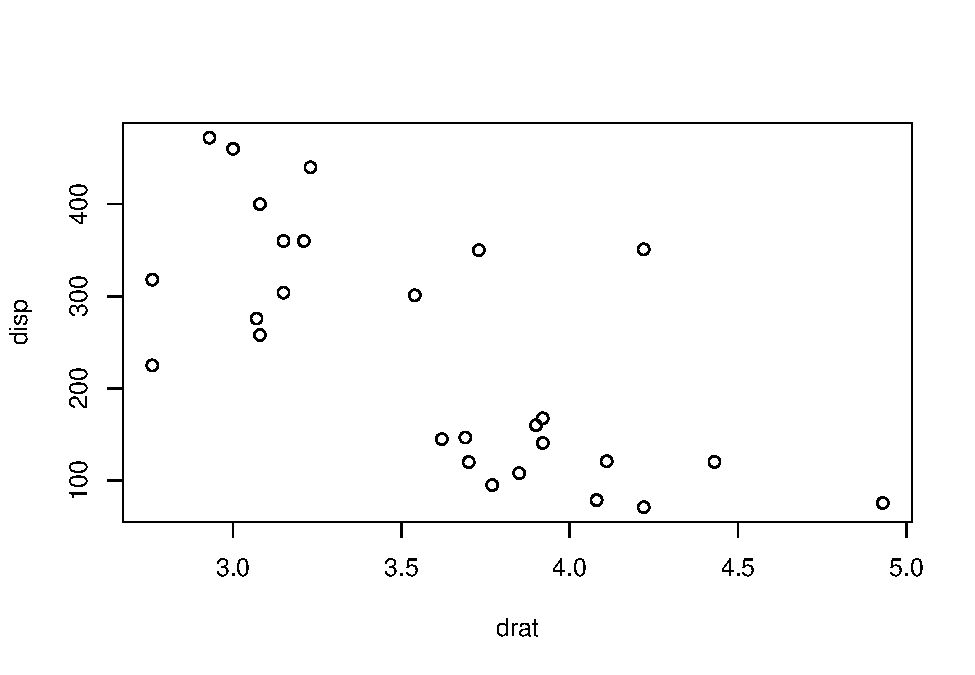
\includegraphics{04.02.01.basic_statistical_analysis_files/figure-latex/unnamed-chunk-3-1.pdf}
-0.71정도로 강한 음의 상관관계가 있음을 알 수 있다.



\paragraph{상관계수와 공분산을 구하자.}\label{--.}

\begin{Shaded}
\begin{Highlighting}[]
\KeywordTok{head}\NormalTok{(}\KeywordTok{cor}\NormalTok{(mtcars))}
\end{Highlighting}
\end{Shaded}

\begin{verbatim}
            mpg        cyl       disp         hp       drat         wt
mpg   1.0000000 -0.8521620 -0.8475514 -0.7761684  0.6811719 -0.8676594
cyl  -0.8521620  1.0000000  0.9020329  0.8324475 -0.6999381  0.7824958
disp -0.8475514  0.9020329  1.0000000  0.7909486 -0.7102139  0.8879799
hp   -0.7761684  0.8324475  0.7909486  1.0000000 -0.4487591  0.6587479
drat  0.6811719 -0.6999381 -0.7102139 -0.4487591  1.0000000 -0.7124406
wt   -0.8676594  0.7824958  0.8879799  0.6587479 -0.7124406  1.0000000
            qsec         vs         am       gear       carb
mpg   0.41868403  0.6640389  0.5998324  0.4802848 -0.5509251
cyl  -0.59124207 -0.8108118 -0.5226070 -0.4926866  0.5269883
disp -0.43369788 -0.7104159 -0.5912270 -0.5555692  0.3949769
hp   -0.70822339 -0.7230967 -0.2432043 -0.1257043  0.7498125
drat  0.09120476  0.4402785  0.7127111  0.6996101 -0.0907898
wt   -0.17471588 -0.5549157 -0.6924953 -0.5832870  0.4276059
그렇다. 
\end{verbatim}
여기에 또 다른 값을 집어넣는다. 


\begin{Shaded}
\begin{Highlighting}[]
\KeywordTok{head}\NormalTok{(}\KeywordTok{cov}\NormalTok{(mtcars))}
\end{Highlighting}
\end{Shaded}

\begin{verbatim}
             mpg         cyl        disp         hp        drat
mpg    36.324103  -9.1723790  -633.09721 -320.73206   2.1950635
cyl    -9.172379   3.1895161   199.66028  101.93145  -0.6683669
disp -633.097208 199.6602823 15360.79983 6721.15867 -47.0640192
hp   -320.732056 101.9314516  6721.15867 4700.86694 -16.4511089
drat    2.195064  -0.6683669   -47.06402  -16.45111   0.2858814
wt     -5.116685   1.3673710   107.68420   44.19266  -0.3727207
              wt         qsec          vs          am        gear
mpg   -5.1166847   4.50914919   2.0171371   1.8039315   2.1356855
cyl    1.3673710  -1.88685484  -0.7298387  -0.4657258  -0.6491935
disp 107.6842040 -96.05168145 -44.3776210 -36.5640121 -50.8026210
hp    44.1926613 -86.77008065 -24.9879032  -8.3205645  -6.3588710
drat  -0.3727207   0.08714073   0.1186492   0.1901512   0.2759879
wt     0.9573790  -0.30548161  -0.2736613  -0.3381048  -0.4210806
            carb
mpg  -5.36310484
cyl   1.52016129
disp 79.06875000
hp   83.03629032
drat -0.07840726
wt    0.67579032
\end{verbatim}

\subsubsection{스피어만 상관계수}\label{-}

\begin{Shaded}
\begin{Highlighting}[]
\KeywordTok{library}\NormalTok{(Hmisc)}
\KeywordTok{rcorr}\NormalTok{(}\KeywordTok{as.matrix}\NormalTok{(mtcars), }\DataTypeTok{type=}\KeywordTok{c}\NormalTok{(}\StringTok{"pearson"}\NormalTok{,}\StringTok{"spearman"}\NormalTok{))}
\end{Highlighting}
\end{Shaded}

\begin{verbatim}
       mpg   cyl  disp    hp  drat    wt  qsec    vs    am  gear  carb
mpg   1.00 -0.85 -0.85 -0.78  0.68 -0.87  0.42  0.66  0.60  0.48 -0.55
cyl  -0.85  1.00  0.90  0.83 -0.70  0.78 -0.59 -0.81 -0.52 -0.49  0.53
disp -0.85  0.90  1.00  0.79 -0.71  0.89 -0.43 -0.71 -0.59 -0.56  0.39
hp   -0.78  0.83  0.79  1.00 -0.45  0.66 -0.71 -0.72 -0.24 -0.13  0.75
drat  0.68 -0.70 -0.71 -0.45  1.00 -0.71  0.09  0.44  0.71  0.70 -0.09
wt   -0.87  0.78  0.89  0.66 -0.71  1.00 -0.17 -0.55 -0.69 -0.58  0.43
qsec  0.42 -0.59 -0.43 -0.71  0.09 -0.17  1.00  0.74 -0.23 -0.21 -0.66
vs    0.66 -0.81 -0.71 -0.72  0.44 -0.55  0.74  1.00  0.17  0.21 -0.57
am    0.60 -0.52 -0.59 -0.24  0.71 -0.69 -0.23  0.17  1.00  0.79  0.06
gear  0.48 -0.49 -0.56 -0.13  0.70 -0.58 -0.21  0.21  0.79  1.00  0.27
carb -0.55  0.53  0.39  0.75 -0.09  0.43 -0.66 -0.57  0.06  0.27  1.00

n= 32 


P
     mpg    cyl    disp   hp     drat   wt     qsec   vs     am     gear  
mpg         0.0000 0.0000 0.0000 0.0000 0.0000 0.0171 0.0000 0.0003 0.0054
cyl  0.0000        0.0000 0.0000 0.0000 0.0000 0.0004 0.0000 0.0022 0.0042
disp 0.0000 0.0000        0.0000 0.0000 0.0000 0.0131 0.0000 0.0004 0.0010
hp   0.0000 0.0000 0.0000        0.0100 0.0000 0.0000 0.0000 0.1798 0.4930
drat 0.0000 0.0000 0.0000 0.0100        0.0000 0.6196 0.0117 0.0000 0.0000
wt   0.0000 0.0000 0.0000 0.0000 0.0000        0.3389 0.0010 0.0000 0.0005
qsec 0.0171 0.0004 0.0131 0.0000 0.6196 0.3389        0.0000 0.2057 0.2425
vs   0.0000 0.0000 0.0000 0.0000 0.0117 0.0010 0.0000        0.3570 0.2579
am   0.0003 0.0022 0.0004 0.1798 0.0000 0.0000 0.2057 0.3570        0.0000
gear 0.0054 0.0042 0.0010 0.4930 0.0000 0.0005 0.2425 0.2579 0.0000       
carb 0.0011 0.0019 0.0253 0.0000 0.6212 0.0146 0.0000 0.0007 0.7545 0.1290
     carb  
mpg  0.0011
cyl  0.0019
disp 0.0253
hp   0.0000
drat 0.6212
wt   0.0146
qsec 0.0000
vs   0.0007
am   0.7545
gear 0.1290
carb       
\end{verbatim}

\paragraph{예제를 풀어보자.}\label{-.}

스피어만 상관계수 행렬을 통해 각변수의 선형적 상관관계를 파악할 수 있다.

\begin{Shaded}
\begin{Highlighting}[]
\NormalTok{studentID <-}\StringTok{ }\KeywordTok{paste}\NormalTok{(}\DecValTok{2009000}\NormalTok{, }\DecValTok{1}\OperatorTok{:}\DecValTok{6}\NormalTok{, }\DataTypeTok{sep=}\StringTok{""}\NormalTok{)}
\NormalTok{Korea <-}\StringTok{ }\KeywordTok{c}\NormalTok{(}\DecValTok{1}\NormalTok{,}\DecValTok{18}\NormalTok{,}\DecValTok{2}\NormalTok{,}\DecValTok{3}\NormalTok{,}\DecValTok{17}\NormalTok{,}\DecValTok{19}\NormalTok{)}
\NormalTok{Math <-}\StringTok{ }\KeywordTok{c}\NormalTok{(}\DecValTok{2}\NormalTok{,}\DecValTok{3}\NormalTok{,}\DecValTok{1}\NormalTok{,}\DecValTok{6}\NormalTok{,}\DecValTok{28}\NormalTok{,}\DecValTok{5}\NormalTok{)}
\NormalTok{Eng <-}\StringTok{ }\KeywordTok{c}\NormalTok{(}\DecValTok{5}\NormalTok{,}\DecValTok{2}\NormalTok{,}\DecValTok{3}\NormalTok{,}\DecValTok{1}\NormalTok{,}\DecValTok{4}\NormalTok{,}\DecValTok{16}\NormalTok{)}
\NormalTok{Science <-}\StringTok{ }\KeywordTok{c}\NormalTok{(}\DecValTok{1}\NormalTok{,}\DecValTok{2}\NormalTok{,}\DecValTok{3}\NormalTok{,}\DecValTok{4}\NormalTok{,}\DecValTok{5}\NormalTok{,}\DecValTok{20}\NormalTok{)}
\NormalTok{test <-}\StringTok{ }\KeywordTok{data.frame}\NormalTok{(studentID,Korea, Math, Eng, Science)}

\KeywordTok{rcorr}\NormalTok{(}\KeywordTok{as.matrix}\NormalTok{(test), }\DataTypeTok{type=}\StringTok{"spearman"}\NormalTok{)}
\end{Highlighting}
\end{Shaded}

\begin{verbatim}
          studentID Korea  Math   Eng Science
studentID      1.00  0.66  0.66  0.26    1.00
Korea          0.66  1.00  0.49  0.14    0.66
Math           0.66  0.49  1.00 -0.09    0.66
Eng            0.26  0.14 -0.09  1.00    0.26
Science        1.00  0.66  0.66  0.26    1.00

n= 6 


P
          studentID Korea  Math   Eng    Science
studentID           0.1562 0.1562 0.6228 0.0000 
Korea     0.1562           0.3287 0.7872 0.1562 
Math      0.1562    0.3287        0.8717 0.1562 
Eng       0.6228    0.7872 0.8717        0.6228 
Science   0.0000    0.1562 0.1562 0.6228        
\end{verbatim}

\subsection{회귀분석}

\subsubsection{단순회귀분석}

예제를 풀어보자 회귀방정식은 \(y= 5.8951 -0.1174x\)로 추정된다.

\begin{Shaded}
\begin{Highlighting}[]
\CommentTok{#난수를 추출하여 임의의 데이터프레임을 만들자}
\KeywordTok{set.seed}\NormalTok{(}\DecValTok{2}\NormalTok{)}
\NormalTok{x=}\KeywordTok{runif}\NormalTok{(}\DecValTok{10}\NormalTok{,}\DecValTok{0}\NormalTok{,}\DecValTok{11}\NormalTok{) ; x}
\end{Highlighting}
\end{Shaded}

\begin{verbatim}
 [1]  2.033705  7.726114  6.306590  1.848571 10.382233 10.378225  1.420749
 [8]  9.167937  5.148204  6.049821
\end{verbatim}

\begin{Shaded}
\begin{Highlighting}[]
\NormalTok{y=}\KeywordTok{runif}\NormalTok{(}\DecValTok{10}\NormalTok{,}\DecValTok{0}\NormalTok{,}\DecValTok{11}\NormalTok{) ;y}
\end{Highlighting}
\end{Shaded}

\begin{verbatim}
 [1]  6.0794147  2.6278424  8.3656464  1.9890211  4.4581040  9.3890330
 [7] 10.7403834  2.4840801  4.8929015  0.8247737
\end{verbatim}

\begin{Shaded}
\begin{Highlighting}[]
\NormalTok{dfrm <-}\StringTok{ }\KeywordTok{data.frame}\NormalTok{(x,y); }\KeywordTok{head}\NormalTok{(dfrm)}
\end{Highlighting}
\end{Shaded}

\begin{verbatim}
          x        y
1  2.033705 6.079415
2  7.726114 2.627842
3  6.306590 8.365646
4  1.848571 1.989021
5 10.382233 4.458104
6 10.378225 9.389033
\end{verbatim}

\begin{Shaded}
\begin{Highlighting}[]
\CommentTok{#회귀분석을 해보자. }
\KeywordTok{lm}\NormalTok{(}\DataTypeTok{formula =}\NormalTok{ y}\OperatorTok{~}\NormalTok{x, }\DataTypeTok{data=}\NormalTok{dfrm) }
\end{Highlighting}
\end{Shaded}

\begin{verbatim}

Call:
lm(formula = y ~ x, data = dfrm)

Coefficients:
(Intercept)            x  
     5.8951      -0.1174  
\end{verbatim}


\end{document}
